\chapter{理論・関連研究}
\label{chap:理論・関連研究}

\section{創造的パートナーシップ}
\label{sec:創造的パートナーシップ}

本節では，人とAIが創造的なパートナーシップを築くために必要な技術的基盤と，解決すべき課題について述べる．

\subsection{エージェントの言語理解と感性}
\label{subsec:エージェントの言語理解}

近年，CLIP\cite{clip}やCLAP\cite{clap}といったマルチモーダル学習モデルの登場により，テキストと画像，あるいはテキストと音声の意味的な対応付けが可能となった．これらは対照学習（Contrastive Learning）を通じて，物理的な対象（「犬」や「ピアノ」など）や一般的な雰囲気（「明るい」「激しい」）に関しては高い精度で認識・生成を行うことができる．

しかし，芸術制作や演奏表現において用いられる言語は，より抽象的で個人的な感性に依存する場合が多い．例えば，「泣くような音色で」や「春の訪れのように」といった表現は，受け手の解釈や文脈によって意味が大きく変化する．
既存のモデルは，一般的なデータセットに基づく平均的な解釈は可能であるが，特定のユーザー固有の感性や，対話の中で形成される動的な文脈（コンテキスト）を理解するには至っていない．エージェントが人のパートナーとして機能するためには，一般的な言語理解を超え，個人の感性に共感的に寄り添う（Alignment）能力が必要とされる．

\subsection{エージェントとの共創と適応学習}
\label{subsec:エージェントとの共創}

ユーザー固有の感性や意図に適応するための技術として，大規模言語モデル（LLM）の文脈内学習能力が注目されている．

\subsubsection{In-context Learning (ICL)}
\label{subsubsec:In-context Learning}
In-context Learning (ICL)\cite{ICL}とは，Brownらによって示されたLLMの能力であり，モデルのパラメータ更新（Fine-tuning）を行わずに，プロンプトとして与えられた入力系列（コンテキスト）のみからタスクの規則やパターンを学習・推論する仕組みを指す．
LLMは事前学習によって獲得した広範な知識とパターン認識能力を活かし，推論時に与えられた数例のデモンストレーションや指示から，即座にタスクに適応することができる．この特性は，ユーザーとの対話履歴を即座に次の生成へと反映させるインタラクティブなシステムにおいて極めて重要である．

\subsubsection{In-context Preference Learning (ICPL)}
\label{subsubsec:In-context Preference Learning}
ICLの概念をさらに発展させ，ユーザーの好み（Preference）を文脈から学習する手法として，\textbf{In-context Preference Learning (ICPL)}\cite{ICPL}が提案されている．
従来，人間の好みに合わせた生成を行うためには，人間のフィードバックに基づく強化学習（RLHF）などが用いられてきたが，これらは学習コストが高く，個々のユーザーに対してリアルタイムに適応することは困難であった．
これに対しICPLは，過去の生成結果に対するユーザーのフィードバック履歴をプロンプトとしてLLMに入力することで，重み更新なしにユーザーの選好を学習する．これにより，対話を重ねるごとにエージェントの出力がユーザーの意図に近づく「すり合わせ」のプロセスを，低コストかつ高速に実現できる（図\ref{fig:ICPL_arch}）．

このICPLは，日高ら\cite{hidaka_ICPL}によって音楽生成（作曲）の分野にも応用されており（図\ref{fig:Hidaka_ICPL_arch}），ユーザーの抽象的な指示を作曲パラメータに変換する際の精度向上に寄与している．本研究では，この仕組みを演奏表現（レンダリング）の制御へと拡張し，人とAIの感性のすり合わせに応用する．

\begin{figure}[t]
    \centering
    \includegraphics[width=1.0\linewidth]{figs/2/ICPL_arch.pdf}
    \caption{ICPLのシステム構成図（\cite{ICPL}より引用）}
    \label{fig:ICPL_arch}
\end{figure}

\begin{figure}[t]
    \centering
    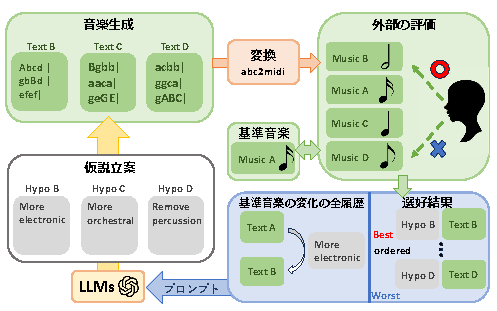
\includegraphics[width=1.0\linewidth]{figs/2/Hidaka_ICPL_arch.pdf}
    \caption{ICPLを作曲AIに応用したシステム構成図（\cite{hidaka_ICPL}より引用）}
    \label{fig:Hidaka_ICPL_arch}
\end{figure}

\begin{figure}[t]
    \centering
    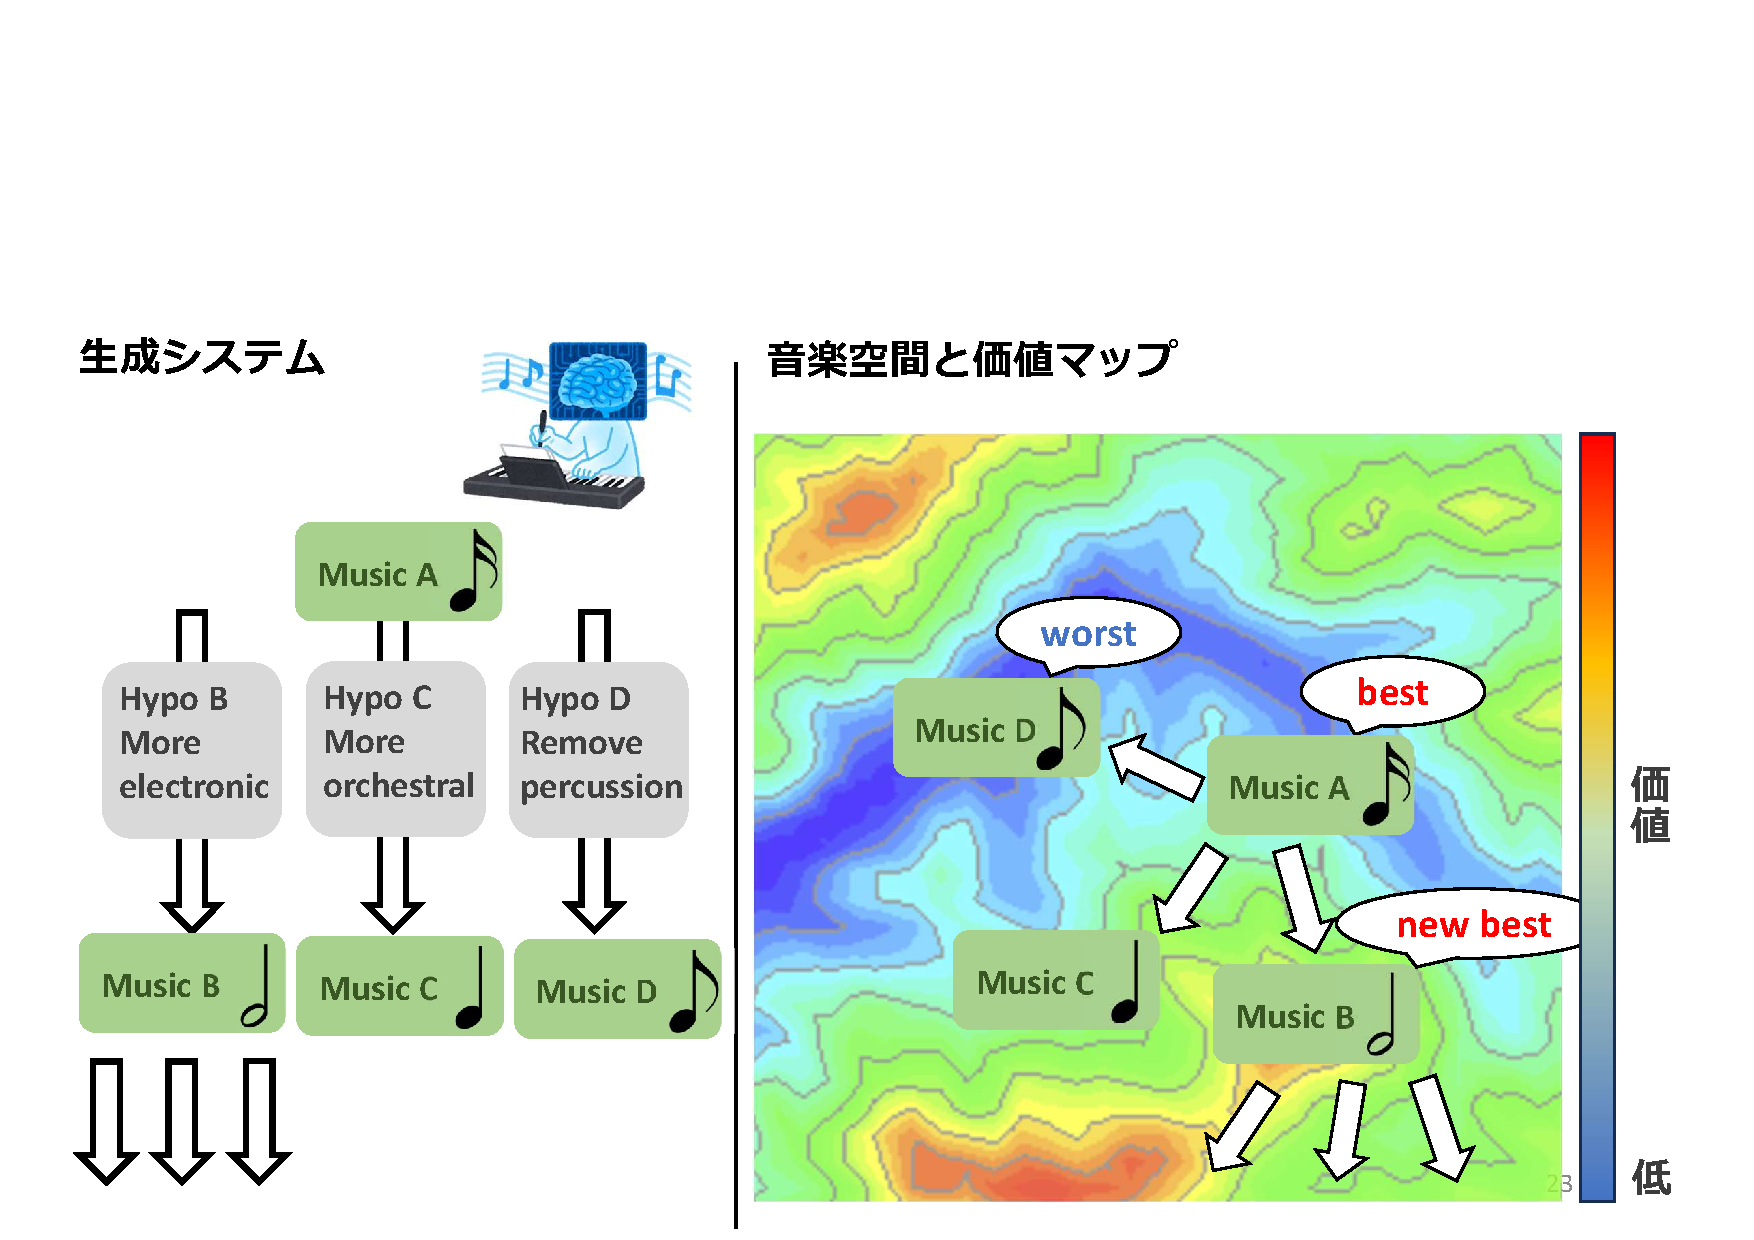
\includegraphics[width=1.0\linewidth]{figs/2/Hidaka_system_image.pdf}
    \caption{ICPLで人の好みを最大化する音楽の探索イメージ（\cite{hidaka_ICPL}より引用）}
    \label{fig:Hidaka_system_image}
\end{figure}

\subsection{AIによる代替と人間の主体性}
\label{subsec:human_creativity}

AIを創造的なパートナーとする際，システムがいかにユーザーの主体性（Agency）を尊重し，創造性を阻害せずに支援できるかは重要な課題である．

\subsubsection{主体性を尊重した最適化支援}
これまでのデザイン支援において，小山らは，ベイズ最適化（Bayesian Optimization）を活用したフレームワーク\cite{BOデザイン提案}を提案している．
従来のデザイン最適化システムでは，システムが生成した案をユーザーに強制的に評価させる（Explicit loop）ものが多く，ユーザーの試行錯誤のプロセスを分断し，主体感を損なう傾向があった．これに対し小山らの手法は，ユーザーがスライダ操作による探索を行っている様子をシステムが「横から観察」し，裏側で非同期的に最適化を行うことで，ユーザーの作業を中断させることなく合理的なデザイン案を提示する．
このアプローチは，ユーザーの自由な探索を阻害しないという点で優れている．しかし，これはあくまでパラメータ空間における数値的な探索支援であり，ユーザーが「どのような意図で」操作しているかという文脈の理解や，言語を通じた相互のコミュニケーションは行われない．すなわち，提示された案を採用するか否かの判断はユーザーに委ねられているものの，そこにはAIとの意味的な対話や共創関係は希薄である．

\subsubsection{LLMとの共創における課題}
一方で，LLMやICPLのような強力な推論・言語能力を持つエージェントとの共創においては，コミュニケーションが可能になる反面，AIが創造プロセスを過度に代替してしまうという新たな課題が生じる．
LLMは膨大な知識量に基づき，対話履歴から高速に最適解らしきものを導き出すことができる（収束的思考）．しかし，Doshiら\cite{人とLLMの共創}による発散的思考と収束的思考に関するランダム化実験では，生成AIがアイデア出しを代替することで，ユーザー自身の思考機会を奪い，かえって創造性を阻害する可能性（Thinking-Halt）が示唆されている．

すなわち，単にユーザーの指示通りに「正解」を出すだけのシステムでは，効率性は向上しても「相互創発的なパートナーシップ」とはなり得ない．AIはユーザーの思考を代替するのではなく，小山らの研究のように主体性を尊重しつつ，多様な選択肢の提示や予期せぬ提案によってユーザーの発散的思考を刺激する役割を担うべきである．
本研究が提案するシステムにおいて，ユーザーによるフィードバックのループ（Human-in-the-loop）を重視し，かつ言語による意図のすり合わせを行うのは，この「主体性の維持」と「意味的な共創」を両立させるためである．


\section{音楽生成における制御と演奏レンダリング}
\label{sec:related_work}

% -----------------------------------------------------------
% 2.1 一般的な生成モデルの話
% -----------------------------------------------------------
\subsection{音楽生成モデルの動向と制御性}
\label{subsec:trends}
近年，深層学習を用いた音楽生成技術は急速に発展している．特に，MusicGen\cite{MusicGen}やMusicLM\cite{MusicLM}などの大規模モデルは，テキストプロンプトから多様なジャンルの楽曲を生成することを可能にした．
しかし，これらのモデルはテキストという抽象的な指示に依存しているため，メロディやリズムといった音楽的な詳細構造（Low-level content）を意図通りに制御することは困難である．Linら\cite{Lin2024}が指摘するように，実用的な音楽制作においては，抽象的なイメージだけでなく，楽譜やMIDIといった具体的な条件付け（Conditioning）に基づく制御が不可欠である．
この課題に対し，近年ではControlNet\cite{ControlNet}やAdapter技術を用い，事前学習済みモデルに追加の制御入力を与える手法が注目されている．

% -----------------------------------------------------------
% 2.2 具体的なタスク（演奏表現）の話
% 最初の画像の論文(2.2 Performance Rendering)の内容を反映
% -----------------------------------------------------------
\subsection{演奏レンダリング (Performance Rendering)}
\label{subsec:performance_rendering}
演奏レンダリングとは，入力された楽譜情報（Score/MIDI）に対し，人間らしい自然な演奏オーディオを生成するタスクである．
これはテキスト読み上げ（TTS）と類似した目的を持つが，音楽特有の多声性（Polyphonic）や，楽譜上の時間と実際の演奏時間の非線形な対応関係（テンポルバート等）により，その難易度は高い．単に楽譜通りの音高・音価を再現するだけでなく，演奏者の解釈による「表現の多様性（Performance Variability）」をいかにモデル化するかが，本タスクにおける重要な課題となっている．

% -----------------------------------------------------------
% 2.3 使用するモデルと数式の話
% -----------------------------------------------------------
\subsection{RenderBoxと基礎理論}
\label{subsec:RenderBox}
本研究では，テキストおよびMIDIによる表現豊かな演奏生成を実現するために，RenderBox\cite{RenderBox}アーキテクチャを採用する．
RenderBoxは，Stable Audio Open\cite{stable-audio-open}を基盤とした潜在拡散モデル（Latent Diffusion Models）であり，そのバックボーンには **DiT (Diffusion Transformer)**\cite{DiT-base} が用いられている．

従来の拡散モデルでは，ノイズ除去ネットワークとしてCNNベースのU-Net\cite{UNet}が標準的に利用されてきた．しかし，U-Netは局所的な特徴抽出に優れる反面，音楽のような長い時系列データにおける大域的な文脈を捉える能力に課題があった．これに対し，Transformer構造を持つDiTは，Self-Attention機構によりデータ全体の依存関係を効率的に学習可能であり，テキストやMIDIといった異なるモダリティの条件付けを柔軟に統合できる利点がある．

また，モデルの学習においては，生成品質と安定性を向上させるために **$v$-objective**\cite{v-prediction} と呼ばれる定式化を採用している．
これは，拡散過程におけるノイズ $\epsilon$ ではなく，速度 $v$ を予測対象とする手法である．時刻 $t$ における潜在変数を $z_t$，ノイズスケジュールに基づく係数を $\alpha_t, \sigma_t$ とすると，ターゲットとなる $v_t$ および損失関数 $\mathcal{L}$ は以下のように定義される．

\begin{align}
    v_t &\equiv \alpha_t \epsilon - \sigma_t z_0 \\
    \mathcal{L} &= \mathbb{E}_{t, z_0, \epsilon} \left[ \| v_t - \hat{v}_\theta(z_t, t, c) \|^2 \right]
\end{align}

ここで $\hat{v}_\theta$ はモデルの出力，$c$ はテキストやMIDIによる条件入力を表す．この手法を採用することで，特にS/N比が低いタイムステップにおける学習が安定し，演奏表現の微細なニュアンスの再現が可能となる．

\begin{figure}[h]
    \centering
    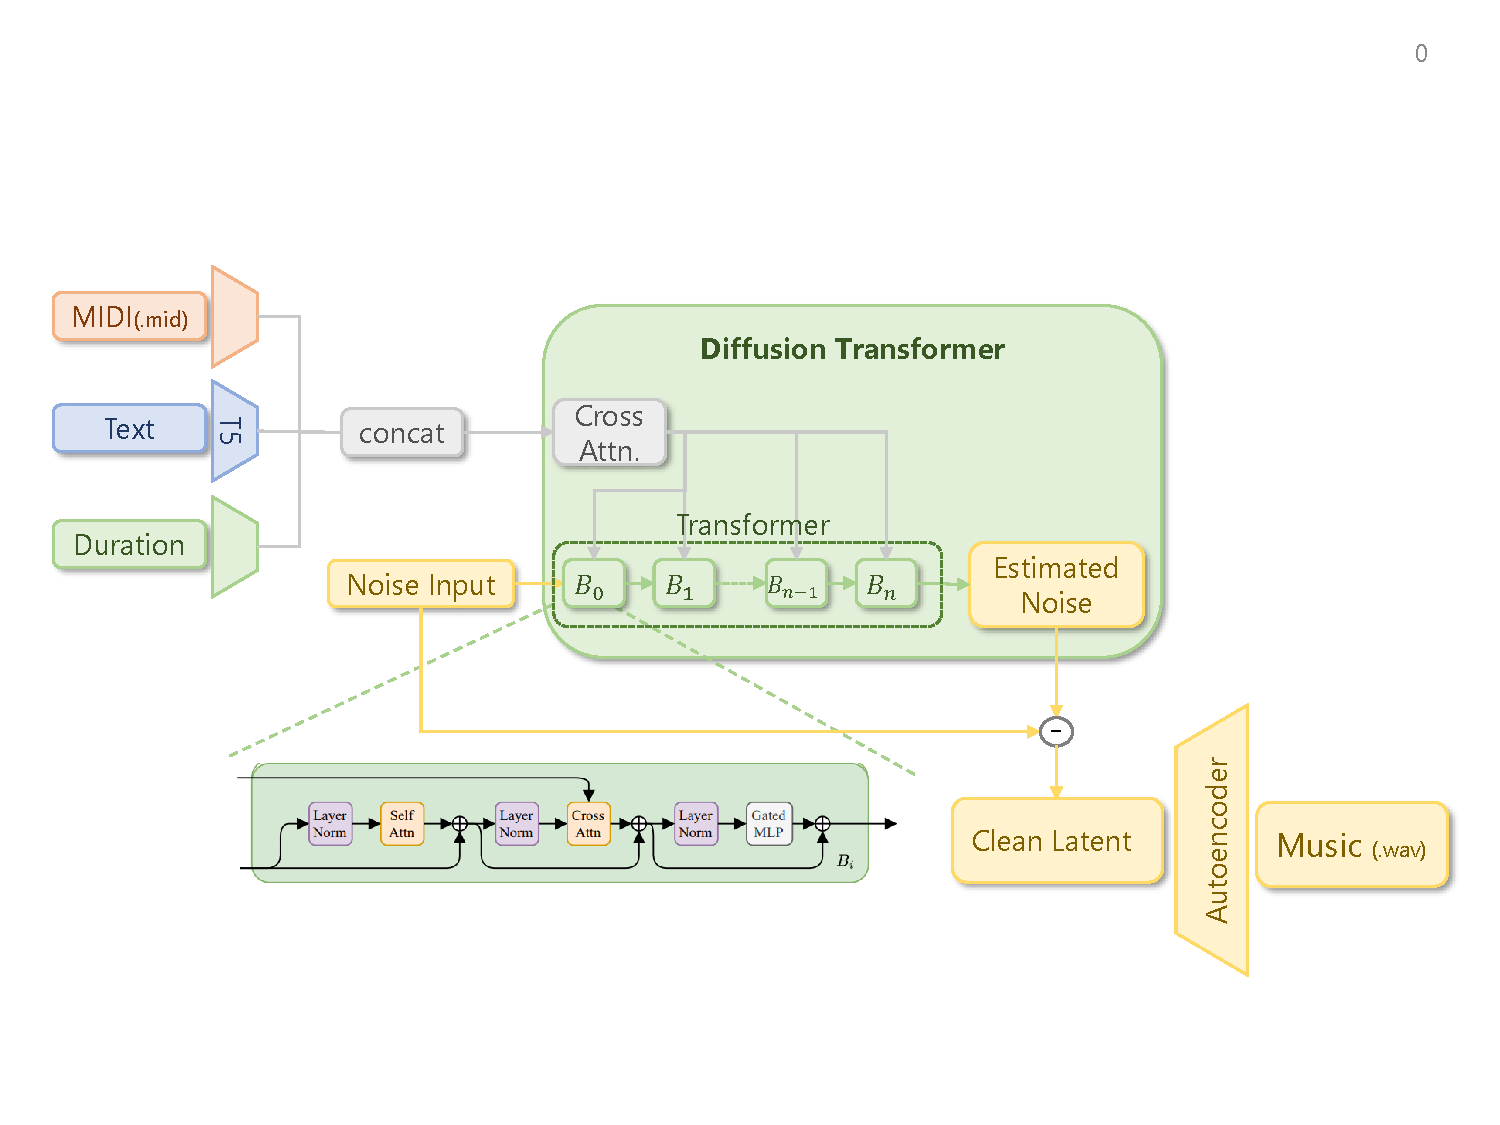
\includegraphics[width=1.0\linewidth]{figs/2/RenderBox_arch.pdf}
    \caption{RenderBoxのアーキテクチャ概要}
    \label{fig:RenderBox_arch}
\end{figure}